\documentclass[]{article}
\usepackage{lmodern}
\usepackage{amssymb,amsmath}
\usepackage{ifxetex,ifluatex}
\usepackage{fixltx2e} % provides \textsubscript
\ifnum 0\ifxetex 1\fi\ifluatex 1\fi=0 % if pdftex
  \usepackage[T1]{fontenc}
  \usepackage[utf8]{inputenc}
\else % if luatex or xelatex
  \ifxetex
    \usepackage{mathspec}
  \else
    \usepackage{fontspec}
  \fi
  \defaultfontfeatures{Ligatures=TeX,Scale=MatchLowercase}
\fi
% use upquote if available, for straight quotes in verbatim environments
\IfFileExists{upquote.sty}{\usepackage{upquote}}{}
% use microtype if available
\IfFileExists{microtype.sty}{%
\usepackage{microtype}
\UseMicrotypeSet[protrusion]{basicmath} % disable protrusion for tt fonts
}{}
\usepackage[margin=1in]{geometry}
\usepackage{hyperref}
\hypersetup{unicode=true,
            pdftitle={DATA 606 Fall 2017 - Final Exam},
            pdfauthor={Joshua Sturm},
            pdfborder={0 0 0},
            breaklinks=true}
\urlstyle{same}  % don't use monospace font for urls
\usepackage{color}
\usepackage{fancyvrb}
\newcommand{\VerbBar}{|}
\newcommand{\VERB}{\Verb[commandchars=\\\{\}]}
\DefineVerbatimEnvironment{Highlighting}{Verbatim}{commandchars=\\\{\}}
% Add ',fontsize=\small' for more characters per line
\usepackage{framed}
\definecolor{shadecolor}{RGB}{248,248,248}
\newenvironment{Shaded}{\begin{snugshade}}{\end{snugshade}}
\newcommand{\KeywordTok}[1]{\textcolor[rgb]{0.13,0.29,0.53}{\textbf{#1}}}
\newcommand{\DataTypeTok}[1]{\textcolor[rgb]{0.13,0.29,0.53}{#1}}
\newcommand{\DecValTok}[1]{\textcolor[rgb]{0.00,0.00,0.81}{#1}}
\newcommand{\BaseNTok}[1]{\textcolor[rgb]{0.00,0.00,0.81}{#1}}
\newcommand{\FloatTok}[1]{\textcolor[rgb]{0.00,0.00,0.81}{#1}}
\newcommand{\ConstantTok}[1]{\textcolor[rgb]{0.00,0.00,0.00}{#1}}
\newcommand{\CharTok}[1]{\textcolor[rgb]{0.31,0.60,0.02}{#1}}
\newcommand{\SpecialCharTok}[1]{\textcolor[rgb]{0.00,0.00,0.00}{#1}}
\newcommand{\StringTok}[1]{\textcolor[rgb]{0.31,0.60,0.02}{#1}}
\newcommand{\VerbatimStringTok}[1]{\textcolor[rgb]{0.31,0.60,0.02}{#1}}
\newcommand{\SpecialStringTok}[1]{\textcolor[rgb]{0.31,0.60,0.02}{#1}}
\newcommand{\ImportTok}[1]{#1}
\newcommand{\CommentTok}[1]{\textcolor[rgb]{0.56,0.35,0.01}{\textit{#1}}}
\newcommand{\DocumentationTok}[1]{\textcolor[rgb]{0.56,0.35,0.01}{\textbf{\textit{#1}}}}
\newcommand{\AnnotationTok}[1]{\textcolor[rgb]{0.56,0.35,0.01}{\textbf{\textit{#1}}}}
\newcommand{\CommentVarTok}[1]{\textcolor[rgb]{0.56,0.35,0.01}{\textbf{\textit{#1}}}}
\newcommand{\OtherTok}[1]{\textcolor[rgb]{0.56,0.35,0.01}{#1}}
\newcommand{\FunctionTok}[1]{\textcolor[rgb]{0.00,0.00,0.00}{#1}}
\newcommand{\VariableTok}[1]{\textcolor[rgb]{0.00,0.00,0.00}{#1}}
\newcommand{\ControlFlowTok}[1]{\textcolor[rgb]{0.13,0.29,0.53}{\textbf{#1}}}
\newcommand{\OperatorTok}[1]{\textcolor[rgb]{0.81,0.36,0.00}{\textbf{#1}}}
\newcommand{\BuiltInTok}[1]{#1}
\newcommand{\ExtensionTok}[1]{#1}
\newcommand{\PreprocessorTok}[1]{\textcolor[rgb]{0.56,0.35,0.01}{\textit{#1}}}
\newcommand{\AttributeTok}[1]{\textcolor[rgb]{0.77,0.63,0.00}{#1}}
\newcommand{\RegionMarkerTok}[1]{#1}
\newcommand{\InformationTok}[1]{\textcolor[rgb]{0.56,0.35,0.01}{\textbf{\textit{#1}}}}
\newcommand{\WarningTok}[1]{\textcolor[rgb]{0.56,0.35,0.01}{\textbf{\textit{#1}}}}
\newcommand{\AlertTok}[1]{\textcolor[rgb]{0.94,0.16,0.16}{#1}}
\newcommand{\ErrorTok}[1]{\textcolor[rgb]{0.64,0.00,0.00}{\textbf{#1}}}
\newcommand{\NormalTok}[1]{#1}
\usepackage{graphicx,grffile}
\makeatletter
\def\maxwidth{\ifdim\Gin@nat@width>\linewidth\linewidth\else\Gin@nat@width\fi}
\def\maxheight{\ifdim\Gin@nat@height>\textheight\textheight\else\Gin@nat@height\fi}
\makeatother
% Scale images if necessary, so that they will not overflow the page
% margins by default, and it is still possible to overwrite the defaults
% using explicit options in \includegraphics[width, height, ...]{}
\setkeys{Gin}{width=\maxwidth,height=\maxheight,keepaspectratio}
\IfFileExists{parskip.sty}{%
\usepackage{parskip}
}{% else
\setlength{\parindent}{0pt}
\setlength{\parskip}{6pt plus 2pt minus 1pt}
}
\setlength{\emergencystretch}{3em}  % prevent overfull lines
\providecommand{\tightlist}{%
  \setlength{\itemsep}{0pt}\setlength{\parskip}{0pt}}
\setcounter{secnumdepth}{0}
% Redefines (sub)paragraphs to behave more like sections
\ifx\paragraph\undefined\else
\let\oldparagraph\paragraph
\renewcommand{\paragraph}[1]{\oldparagraph{#1}\mbox{}}
\fi
\ifx\subparagraph\undefined\else
\let\oldsubparagraph\subparagraph
\renewcommand{\subparagraph}[1]{\oldsubparagraph{#1}\mbox{}}
\fi

%%% Use protect on footnotes to avoid problems with footnotes in titles
\let\rmarkdownfootnote\footnote%
\def\footnote{\protect\rmarkdownfootnote}

%%% Change title format to be more compact
\usepackage{titling}

% Create subtitle command for use in maketitle
\newcommand{\subtitle}[1]{
  \posttitle{
    \begin{center}\large#1\end{center}
    }
}

\setlength{\droptitle}{-2em}
  \title{DATA 606 Fall 2017 - Final Exam}
  \pretitle{\vspace{\droptitle}\centering\huge}
  \posttitle{\par}
  \author{Joshua Sturm}
  \preauthor{\centering\large\emph}
  \postauthor{\par}
  \date{}
  \predate{}\postdate{}


\begin{document}
\maketitle

\section{Part I}\label{part-i}

Please put the answers for Part I next to the question number (2pts
each):

\begin{enumerate}
\def\labelenumi{\arabic{enumi}.}
\tightlist
\item
  B. Quantitative - counts, discrete - whole numbers.
\item
  A. Since the histogram is left-skewed, we can assume that the median
  is larger than the mean. Between a, c, and e, a seems the most
  realistic.
\item
  A. B is an observational study, and cannot be used to draw causality
  inferences.
\item
  D. A large chi-square test means the data is ill-fitted, and there is
  no relationship.
\item
  B. We have the formulas \(Q_1 - IQR\cdot1.5\) and
  \(Q_3 + IQR\cdot1.5\).
\end{enumerate}

\begin{Shaded}
\begin{Highlighting}[]
\NormalTok{q1 <-}\StringTok{ }\DecValTok{37}
\NormalTok{q3 <-}\StringTok{ }\FloatTok{49.8}
\NormalTok{iqr <-}\StringTok{ }\NormalTok{q3 }\OperatorTok{-}\StringTok{ }\NormalTok{q1}
\NormalTok{iqr.}\DecValTok{15}\NormalTok{ <-}\StringTok{ }\FloatTok{1.5} \OperatorTok{*}\StringTok{ }\NormalTok{iqr}
\NormalTok{q1 }\OperatorTok{-}\StringTok{ }\NormalTok{iqr.}\DecValTok{15}
\end{Highlighting}
\end{Shaded}

\begin{verbatim}
## [1] 17.8
\end{verbatim}

\begin{Shaded}
\begin{Highlighting}[]
\NormalTok{q3 }\OperatorTok{+}\StringTok{ }\NormalTok{iqr.}\DecValTok{15}
\end{Highlighting}
\end{Shaded}

\begin{verbatim}
## [1] 69
\end{verbatim}

\begin{enumerate}
\def\labelenumi{\arabic{enumi}.}
\setcounter{enumi}{5}
\item
  \begin{enumerate}
  \def\labelenumii{\Alph{enumii}.}
  \setcounter{enumii}{3}
  \item
  \end{enumerate}
\end{enumerate}

7a. Describe the two distributions (2pts).

\emph{A} - Unimodal, right-skewed, nearly-normal.

\emph{B} - unimodal, symmetrical, nearly-normal.

7b. Explain why the means of these two distributions are similar but the
standard deviations are not (2 pts).

Since B has many, random, independent samples from A, it will be nearly
normal, and have a similar mean. With fewer samples, there is more
spread, and samples farther from the mean. The formula for the SD in B
is \(\frac{sd}{\sqrt{n}}\).

7c. What is the statistical principal that describes this phenomenon (2
pts)?

This is known as the Central Limit Theorem. If the sample size is
greater than 30, each one being independent of the other, and no
significant skew, it follows (converges toward) a normal distribution.

\section{Part II}\label{part-ii}

Consider the four datasets, each with two columns (x and y), provided
below.

\begin{Shaded}
\begin{Highlighting}[]
\CommentTok{#options(digits=2)}
\KeywordTok{options}\NormalTok{(}\DataTypeTok{digits=}\DecValTok{10}\NormalTok{)}
\NormalTok{data1 <-}\StringTok{ }\KeywordTok{data.frame}\NormalTok{(}\DataTypeTok{x=}\KeywordTok{c}\NormalTok{(}\DecValTok{10}\NormalTok{,}\DecValTok{8}\NormalTok{,}\DecValTok{13}\NormalTok{,}\DecValTok{9}\NormalTok{,}\DecValTok{11}\NormalTok{,}\DecValTok{14}\NormalTok{,}\DecValTok{6}\NormalTok{,}\DecValTok{4}\NormalTok{,}\DecValTok{12}\NormalTok{,}\DecValTok{7}\NormalTok{,}\DecValTok{5}\NormalTok{),}
                    \DataTypeTok{y=}\KeywordTok{c}\NormalTok{(}\FloatTok{8.04}\NormalTok{,}\FloatTok{6.95}\NormalTok{,}\FloatTok{7.58}\NormalTok{,}\FloatTok{8.81}\NormalTok{,}\FloatTok{8.33}\NormalTok{,}\FloatTok{9.96}\NormalTok{,}\FloatTok{7.24}\NormalTok{,}\FloatTok{4.26}\NormalTok{,}\FloatTok{10.84}\NormalTok{,}\FloatTok{4.82}\NormalTok{,}\FloatTok{5.68}\NormalTok{))}
\NormalTok{data2 <-}\StringTok{ }\KeywordTok{data.frame}\NormalTok{(}\DataTypeTok{x=}\KeywordTok{c}\NormalTok{(}\DecValTok{10}\NormalTok{,}\DecValTok{8}\NormalTok{,}\DecValTok{13}\NormalTok{,}\DecValTok{9}\NormalTok{,}\DecValTok{11}\NormalTok{,}\DecValTok{14}\NormalTok{,}\DecValTok{6}\NormalTok{,}\DecValTok{4}\NormalTok{,}\DecValTok{12}\NormalTok{,}\DecValTok{7}\NormalTok{,}\DecValTok{5}\NormalTok{),}
                    \DataTypeTok{y=}\KeywordTok{c}\NormalTok{(}\FloatTok{9.14}\NormalTok{,}\FloatTok{8.14}\NormalTok{,}\FloatTok{8.74}\NormalTok{,}\FloatTok{8.77}\NormalTok{,}\FloatTok{9.26}\NormalTok{,}\FloatTok{8.1}\NormalTok{,}\FloatTok{6.13}\NormalTok{,}\FloatTok{3.1}\NormalTok{,}\FloatTok{9.13}\NormalTok{,}\FloatTok{7.26}\NormalTok{,}\FloatTok{4.74}\NormalTok{))}
\NormalTok{data3 <-}\StringTok{ }\KeywordTok{data.frame}\NormalTok{(}\DataTypeTok{x=}\KeywordTok{c}\NormalTok{(}\DecValTok{10}\NormalTok{,}\DecValTok{8}\NormalTok{,}\DecValTok{13}\NormalTok{,}\DecValTok{9}\NormalTok{,}\DecValTok{11}\NormalTok{,}\DecValTok{14}\NormalTok{,}\DecValTok{6}\NormalTok{,}\DecValTok{4}\NormalTok{,}\DecValTok{12}\NormalTok{,}\DecValTok{7}\NormalTok{,}\DecValTok{5}\NormalTok{),}
                    \DataTypeTok{y=}\KeywordTok{c}\NormalTok{(}\FloatTok{7.46}\NormalTok{,}\FloatTok{6.77}\NormalTok{,}\FloatTok{12.74}\NormalTok{,}\FloatTok{7.11}\NormalTok{,}\FloatTok{7.81}\NormalTok{,}\FloatTok{8.84}\NormalTok{,}\FloatTok{6.08}\NormalTok{,}\FloatTok{5.39}\NormalTok{,}\FloatTok{8.15}\NormalTok{,}\FloatTok{6.42}\NormalTok{,}\FloatTok{5.73}\NormalTok{))}
\NormalTok{data4 <-}\StringTok{ }\KeywordTok{data.frame}\NormalTok{(}\DataTypeTok{x=}\KeywordTok{c}\NormalTok{(}\DecValTok{8}\NormalTok{,}\DecValTok{8}\NormalTok{,}\DecValTok{8}\NormalTok{,}\DecValTok{8}\NormalTok{,}\DecValTok{8}\NormalTok{,}\DecValTok{8}\NormalTok{,}\DecValTok{8}\NormalTok{,}\DecValTok{19}\NormalTok{,}\DecValTok{8}\NormalTok{,}\DecValTok{8}\NormalTok{,}\DecValTok{8}\NormalTok{),}
                    \DataTypeTok{y=}\KeywordTok{c}\NormalTok{(}\FloatTok{6.58}\NormalTok{,}\FloatTok{5.76}\NormalTok{,}\FloatTok{7.71}\NormalTok{,}\FloatTok{8.84}\NormalTok{,}\FloatTok{8.47}\NormalTok{,}\FloatTok{7.04}\NormalTok{,}\FloatTok{5.25}\NormalTok{,}\FloatTok{12.5}\NormalTok{,}\FloatTok{5.56}\NormalTok{,}\FloatTok{7.91}\NormalTok{,}\FloatTok{6.89}\NormalTok{))}
\end{Highlighting}
\end{Shaded}

For each column, calculate (to two decimal places):

\paragraph{a. The mean (for x and y separately; 1
pt).}\label{a.-the-mean-for-x-and-y-separately-1-pt.}

\begin{Shaded}
\begin{Highlighting}[]
\CommentTok{#}
\CommentTok{# These may not be the most efficient way. Also, I would put them into a dataframe, or nicer display output}
\CommentTok{#}
\NormalTok{mean =}\StringTok{ }\KeywordTok{lapply}\NormalTok{(}
  \KeywordTok{c}\NormalTok{(data1, data2, data3, data4),}
  \ControlFlowTok{function}\NormalTok{(x) }
\NormalTok{  \{}
\NormalTok{    y <-}\StringTok{ }\KeywordTok{mean}\NormalTok{(x)}
    \KeywordTok{round}\NormalTok{(y, }\DecValTok{2}\NormalTok{)}
\NormalTok{  \}}
\NormalTok{)}
\NormalTok{mean}
\end{Highlighting}
\end{Shaded}

\begin{verbatim}
## $x
## [1] 9
## 
## $y
## [1] 7.5
## 
## $x
## [1] 9
## 
## $y
## [1] 7.5
## 
## $x
## [1] 9
## 
## $y
## [1] 7.5
## 
## $x
## [1] 9
## 
## $y
## [1] 7.5
\end{verbatim}

\paragraph{b. The median (for x and y separately; 1
pt).}\label{b.-the-median-for-x-and-y-separately-1-pt.}

\begin{Shaded}
\begin{Highlighting}[]
\NormalTok{median =}\StringTok{ }\KeywordTok{lapply}\NormalTok{(}
  \KeywordTok{c}\NormalTok{(data1, data2, data3, data4),}
  \ControlFlowTok{function}\NormalTok{(x) }
\NormalTok{  \{}
\NormalTok{    y <-}\StringTok{ }\KeywordTok{median}\NormalTok{(x)}
    \KeywordTok{round}\NormalTok{(y, }\DecValTok{2}\NormalTok{)}
\NormalTok{  \}}
\NormalTok{)}
\NormalTok{median}
\end{Highlighting}
\end{Shaded}

\begin{verbatim}
## $x
## [1] 9
## 
## $y
## [1] 7.58
## 
## $x
## [1] 9
## 
## $y
## [1] 8.14
## 
## $x
## [1] 9
## 
## $y
## [1] 7.11
## 
## $x
## [1] 8
## 
## $y
## [1] 7.04
\end{verbatim}

\paragraph{c. The standard deviation (for x and y separately; 1
pt).}\label{c.-the-standard-deviation-for-x-and-y-separately-1-pt.}

\begin{Shaded}
\begin{Highlighting}[]
\NormalTok{sd =}\StringTok{ }\KeywordTok{lapply}\NormalTok{(}
  \KeywordTok{c}\NormalTok{(data1, data2, data3, data4),}
  \ControlFlowTok{function}\NormalTok{(x) }
\NormalTok{  \{}
\NormalTok{    y <-}\StringTok{ }\KeywordTok{sd}\NormalTok{(x)}
    \KeywordTok{round}\NormalTok{(y, }\DecValTok{2}\NormalTok{)}
\NormalTok{  \}}
\NormalTok{)}
\NormalTok{sd}
\end{Highlighting}
\end{Shaded}

\begin{verbatim}
## $x
## [1] 3.32
## 
## $y
## [1] 2.03
## 
## $x
## [1] 3.32
## 
## $y
## [1] 2.03
## 
## $x
## [1] 3.32
## 
## $y
## [1] 2.03
## 
## $x
## [1] 3.32
## 
## $y
## [1] 2.03
\end{verbatim}

\paragraph{For each x and y pair, calculate (also to two decimal places;
1
pt):}\label{for-each-x-and-y-pair-calculate-also-to-two-decimal-places-1-pt}

\paragraph{d. The correlation (1 pt).}\label{d.-the-correlation-1-pt.}

\begin{Shaded}
\begin{Highlighting}[]
\KeywordTok{round}\NormalTok{(}\KeywordTok{cor}\NormalTok{(data1), }\DecValTok{2}\NormalTok{)}
\end{Highlighting}
\end{Shaded}

\begin{verbatim}
##      x    y
## x 1.00 0.82
## y 0.82 1.00
\end{verbatim}

\begin{Shaded}
\begin{Highlighting}[]
\KeywordTok{round}\NormalTok{(}\KeywordTok{cor}\NormalTok{(data2), }\DecValTok{2}\NormalTok{)}
\end{Highlighting}
\end{Shaded}

\begin{verbatim}
##      x    y
## x 1.00 0.82
## y 0.82 1.00
\end{verbatim}

\begin{Shaded}
\begin{Highlighting}[]
\KeywordTok{round}\NormalTok{(}\KeywordTok{cor}\NormalTok{(data3), }\DecValTok{2}\NormalTok{)}
\end{Highlighting}
\end{Shaded}

\begin{verbatim}
##      x    y
## x 1.00 0.82
## y 0.82 1.00
\end{verbatim}

\begin{Shaded}
\begin{Highlighting}[]
\KeywordTok{round}\NormalTok{(}\KeywordTok{cor}\NormalTok{(data4), }\DecValTok{2}\NormalTok{)}
\end{Highlighting}
\end{Shaded}

\begin{verbatim}
##      x    y
## x 1.00 0.82
## y 0.82 1.00
\end{verbatim}

\paragraph{e. Linear regression equation (2
pts).}\label{e.-linear-regression-equation-2-pts.}

\begin{Shaded}
\begin{Highlighting}[]
\KeywordTok{par}\NormalTok{(}\DataTypeTok{mfrow =} \KeywordTok{c}\NormalTok{(}\DecValTok{2}\NormalTok{, }\DecValTok{2}\NormalTok{))}
\NormalTok{lr1 <-}\StringTok{ }\KeywordTok{lm}\NormalTok{(y }\OperatorTok{~}\StringTok{ }\NormalTok{x, data1)}
\KeywordTok{print}\NormalTok{(}\KeywordTok{summary}\NormalTok{(lr1), }\KeywordTok{round}\NormalTok{(}\DecValTok{2}\NormalTok{))}
\end{Highlighting}
\end{Shaded}

\begin{verbatim}
## 
## Call:
## lm(formula = y ~ x, data = data1)
## 
## Residuals:
##    Min     1Q Median     3Q    Max 
## -1.921 -0.456 -0.041  0.709  1.839 
## 
## Coefficients:
##             Estimate Std. Error t value Pr(>|t|)   
## (Intercept)     3.00       1.12     2.7    0.026 * 
## x               0.50       0.12     4.2    0.002 **
## ---
## Signif. codes:  0 '***' 0.001 '**' 0.01 '*' 0.05 '.' 0.1 ' ' 1
## 
## Residual standard error: 1.2 on 9 degrees of freedom
## Multiple R-squared:  0.67,   Adjusted R-squared:  0.63 
## F-statistic:  18 on 1 and 9 DF,  p-value: 0.0022
\end{verbatim}

\begin{Shaded}
\begin{Highlighting}[]
\KeywordTok{plot}\NormalTok{(lr1)}
\end{Highlighting}
\end{Shaded}

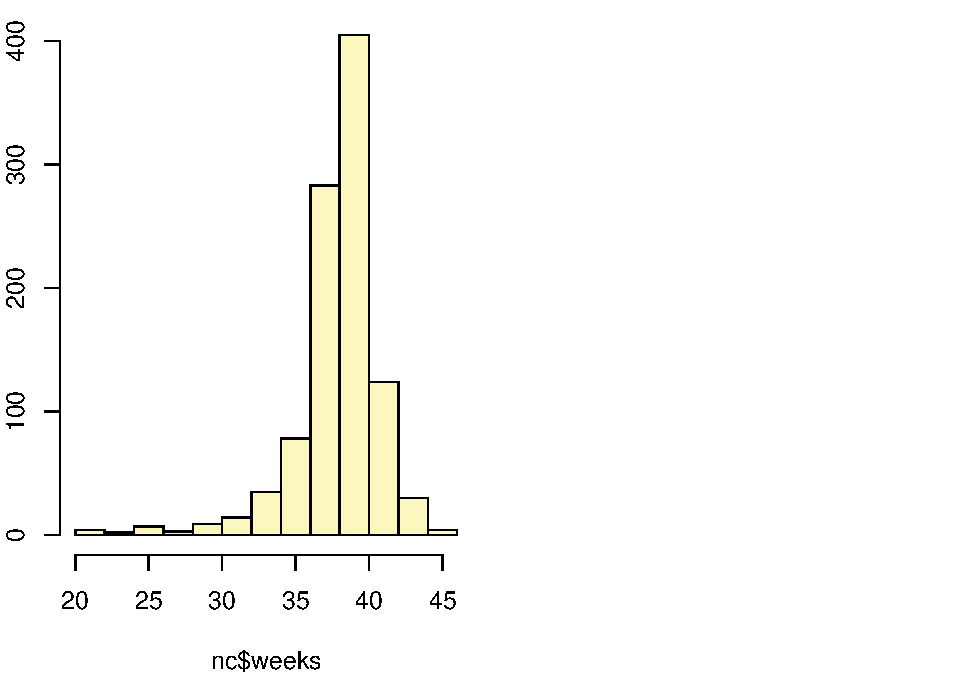
\includegraphics{Final_Exam_Answers_files/figure-latex/unnamed-chunk-7-1.pdf}

\begin{Shaded}
\begin{Highlighting}[]
\NormalTok{lr2 <-}\StringTok{ }\KeywordTok{lm}\NormalTok{(y }\OperatorTok{~}\StringTok{ }\NormalTok{x, data2)}
\KeywordTok{print}\NormalTok{(}\KeywordTok{summary}\NormalTok{(lr2), }\KeywordTok{round}\NormalTok{(}\DecValTok{2}\NormalTok{))}
\end{Highlighting}
\end{Shaded}

\begin{verbatim}
## 
## Call:
## lm(formula = y ~ x, data = data2)
## 
## Residuals:
##    Min     1Q Median     3Q    Max 
##  -1.90  -0.76   0.13   0.95   1.27 
## 
## Coefficients:
##             Estimate Std. Error t value Pr(>|t|)   
## (Intercept)     3.00       1.13     2.7    0.026 * 
## x               0.50       0.12     4.2    0.002 **
## ---
## Signif. codes:  0 '***' 0.001 '**' 0.01 '*' 0.05 '.' 0.1 ' ' 1
## 
## Residual standard error: 1.2 on 9 degrees of freedom
## Multiple R-squared:  0.67,   Adjusted R-squared:  0.63 
## F-statistic:  18 on 1 and 9 DF,  p-value: 0.0022
\end{verbatim}

\begin{Shaded}
\begin{Highlighting}[]
\KeywordTok{plot}\NormalTok{(lr2)}
\end{Highlighting}
\end{Shaded}

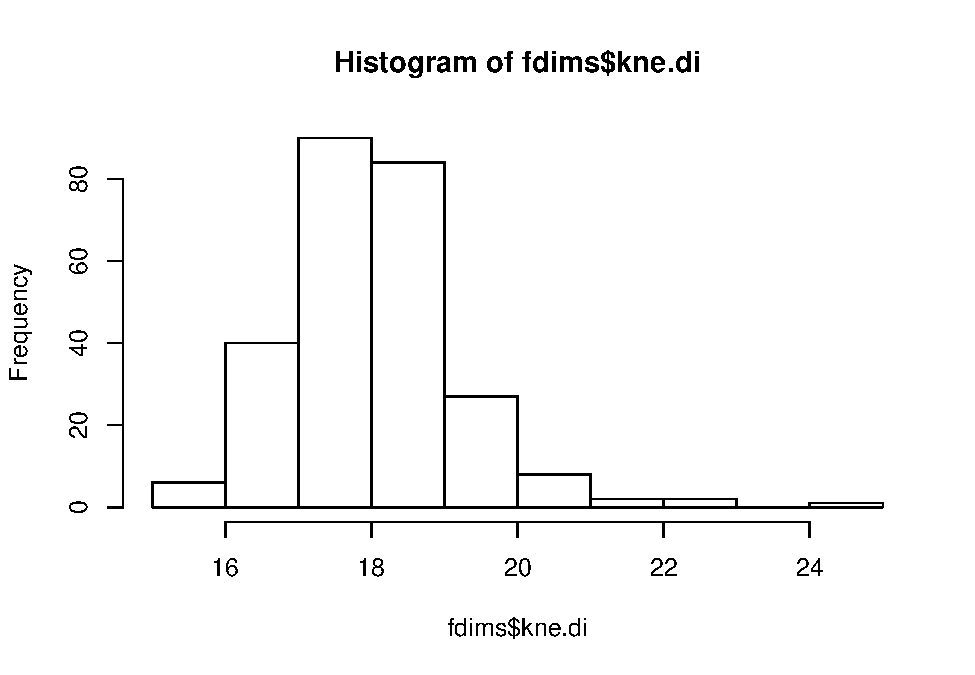
\includegraphics{Final_Exam_Answers_files/figure-latex/unnamed-chunk-7-2.pdf}

\begin{Shaded}
\begin{Highlighting}[]
\NormalTok{lr3 <-}\StringTok{ }\KeywordTok{lm}\NormalTok{(y }\OperatorTok{~}\StringTok{ }\NormalTok{x, data3)}
\KeywordTok{print}\NormalTok{(}\KeywordTok{summary}\NormalTok{(lr3), }\KeywordTok{round}\NormalTok{(}\DecValTok{2}\NormalTok{))}
\end{Highlighting}
\end{Shaded}

\begin{verbatim}
## 
## Call:
## lm(formula = y ~ x, data = data3)
## 
## Residuals:
##    Min     1Q Median     3Q    Max 
##  -1.16  -0.61  -0.23   0.15   3.24 
## 
## Coefficients:
##             Estimate Std. Error t value Pr(>|t|)   
## (Intercept)     3.00       1.12     2.7    0.026 * 
## x               0.50       0.12     4.2    0.002 **
## ---
## Signif. codes:  0 '***' 0.001 '**' 0.01 '*' 0.05 '.' 0.1 ' ' 1
## 
## Residual standard error: 1.2 on 9 degrees of freedom
## Multiple R-squared:  0.67,   Adjusted R-squared:  0.63 
## F-statistic:  18 on 1 and 9 DF,  p-value: 0.0022
\end{verbatim}

\begin{Shaded}
\begin{Highlighting}[]
\KeywordTok{plot}\NormalTok{(lr3)}
\end{Highlighting}
\end{Shaded}

\includegraphics{Final_Exam_Answers_files/figure-latex/unnamed-chunk-7-3.pdf}

\begin{Shaded}
\begin{Highlighting}[]
\NormalTok{lr4 <-}\StringTok{ }\KeywordTok{lm}\NormalTok{(y }\OperatorTok{~}\StringTok{ }\NormalTok{x, data4)}
\KeywordTok{print}\NormalTok{(}\KeywordTok{summary}\NormalTok{(lr4), }\KeywordTok{round}\NormalTok{(}\DecValTok{2}\NormalTok{))}
\end{Highlighting}
\end{Shaded}

\begin{verbatim}
## 
## Call:
## lm(formula = y ~ x, data = data4)
## 
## Residuals:
##    Min     1Q Median     3Q    Max 
##  -1.75  -0.83   0.00   0.81   1.84 
## 
## Coefficients:
##             Estimate Std. Error t value Pr(>|t|)   
## (Intercept)     3.00       1.12     2.7    0.026 * 
## x               0.50       0.12     4.2    0.002 **
## ---
## Signif. codes:  0 '***' 0.001 '**' 0.01 '*' 0.05 '.' 0.1 ' ' 1
## 
## Residual standard error: 1.2 on 9 degrees of freedom
## Multiple R-squared:  0.67,   Adjusted R-squared:  0.63 
## F-statistic:  18 on 1 and 9 DF,  p-value: 0.0022
\end{verbatim}

\begin{Shaded}
\begin{Highlighting}[]
\KeywordTok{plot}\NormalTok{(lr4)}
\end{Highlighting}
\end{Shaded}

\begin{verbatim}
## Warning: not plotting observations with leverage one:
##   8

## Warning: not plotting observations with leverage one:
##   8
\end{verbatim}

\includegraphics{Final_Exam_Answers_files/figure-latex/unnamed-chunk-7-4.pdf}

\paragraph{f. R-Squared (2 pts).}\label{f.-r-squared-2-pts.}

\begin{Shaded}
\begin{Highlighting}[]
\KeywordTok{print}\NormalTok{(}\KeywordTok{summary}\NormalTok{(lr1)}\OperatorTok{$}\NormalTok{r.squared, }\KeywordTok{round}\NormalTok{(}\DecValTok{2}\NormalTok{))}
\end{Highlighting}
\end{Shaded}

\begin{verbatim}
## [1] 0.67
\end{verbatim}

\begin{Shaded}
\begin{Highlighting}[]
\KeywordTok{print}\NormalTok{(}\KeywordTok{summary}\NormalTok{(lr2)}\OperatorTok{$}\NormalTok{r.squared, }\KeywordTok{round}\NormalTok{(}\DecValTok{2}\NormalTok{))}
\end{Highlighting}
\end{Shaded}

\begin{verbatim}
## [1] 0.67
\end{verbatim}

\begin{Shaded}
\begin{Highlighting}[]
\KeywordTok{print}\NormalTok{(}\KeywordTok{summary}\NormalTok{(lr3)}\OperatorTok{$}\NormalTok{r.squared, }\KeywordTok{round}\NormalTok{(}\DecValTok{2}\NormalTok{))}
\end{Highlighting}
\end{Shaded}

\begin{verbatim}
## [1] 0.67
\end{verbatim}

\begin{Shaded}
\begin{Highlighting}[]
\KeywordTok{print}\NormalTok{(}\KeywordTok{summary}\NormalTok{(lr4)}\OperatorTok{$}\NormalTok{r.squared, }\KeywordTok{round}\NormalTok{(}\DecValTok{2}\NormalTok{))}
\end{Highlighting}
\end{Shaded}

\begin{verbatim}
## [1] 0.67
\end{verbatim}

\paragraph{For each pair, is it appropriate to estimate a linear
regression model? Why or why not? Be specific as to why for each pair
and include appropriate plots! (4
pts)}\label{for-each-pair-is-it-appropriate-to-estimate-a-linear-regression-model-why-or-why-not-be-specific-as-to-why-for-each-pair-and-include-appropriate-plots-4-pts}

There are four requirements for linear regression: - Linearity - Nearly
normal residuals - Constant Variability - Independent observations

\begin{Shaded}
\begin{Highlighting}[]
\KeywordTok{plot}\NormalTok{(data1, }\DataTypeTok{main =}\StringTok{'data1'}\NormalTok{)}
\end{Highlighting}
\end{Shaded}

\includegraphics{Final_Exam_Answers_files/figure-latex/unnamed-chunk-9-1.pdf}

\begin{Shaded}
\begin{Highlighting}[]
\KeywordTok{hist}\NormalTok{(lr1}\OperatorTok{$}\NormalTok{residuals)}
\end{Highlighting}
\end{Shaded}

\includegraphics{Final_Exam_Answers_files/figure-latex/unnamed-chunk-9-2.pdf}

\begin{Shaded}
\begin{Highlighting}[]
\KeywordTok{plot}\NormalTok{(data2, }\DataTypeTok{main =} \StringTok{'data2'}\NormalTok{)}
\end{Highlighting}
\end{Shaded}

\includegraphics{Final_Exam_Answers_files/figure-latex/unnamed-chunk-9-3.pdf}

\begin{Shaded}
\begin{Highlighting}[]
\KeywordTok{hist}\NormalTok{(lr2}\OperatorTok{$}\NormalTok{residuals)}
\end{Highlighting}
\end{Shaded}

\includegraphics{Final_Exam_Answers_files/figure-latex/unnamed-chunk-9-4.pdf}

\begin{Shaded}
\begin{Highlighting}[]
\KeywordTok{plot}\NormalTok{(data3, }\DataTypeTok{main =} \StringTok{'data3'}\NormalTok{)}
\end{Highlighting}
\end{Shaded}

\includegraphics{Final_Exam_Answers_files/figure-latex/unnamed-chunk-9-5.pdf}

\begin{Shaded}
\begin{Highlighting}[]
\KeywordTok{hist}\NormalTok{(lr3}\OperatorTok{$}\NormalTok{residuals)}
\end{Highlighting}
\end{Shaded}

\includegraphics{Final_Exam_Answers_files/figure-latex/unnamed-chunk-9-6.pdf}

\begin{Shaded}
\begin{Highlighting}[]
\KeywordTok{plot}\NormalTok{(data4, }\DataTypeTok{main =} \StringTok{'data4'}\NormalTok{)}
\end{Highlighting}
\end{Shaded}

\includegraphics{Final_Exam_Answers_files/figure-latex/unnamed-chunk-9-7.pdf}

\begin{Shaded}
\begin{Highlighting}[]
\KeywordTok{hist}\NormalTok{(lr4}\OperatorTok{$}\NormalTok{residuals)}
\end{Highlighting}
\end{Shaded}

\includegraphics{Final_Exam_Answers_files/figure-latex/unnamed-chunk-9-8.pdf}

\begin{itemize}
\tightlist
\item
  \emph{Dataset 1}: Plot seems normal, but the residuals are not.
\item
  \emph{Dataset 2}: Plot is not linear, and residuals are not normal.
\item
  \emph{Dataset 3}: Seems normal, except for the outlier, which skews
  the histogram.
\item
  \emph{Dataset 4}: No variability in the plot, and also has an outlier.
\end{itemize}

If any of the four were apropriate for linear regression, I'd go with
three.

\paragraph{Explain why it is important to include appropriate
visualizations when analyzing data. Include any visualization(s) you
create. (2
pts)}\label{explain-why-it-is-important-to-include-appropriate-visualizations-when-analyzing-data.-include-any-visualizations-you-create.-2-pts}

If you want a quick idea of the subject without delving into the
numbers, it's easy to look at a graph. Also, you can spot things you
might miss in the numbers, e.g.~the outliers. Visualizations are also a
good way to summarize a lot of information in a clean, concise,
understandable format. Lastly, many people are visual learners. They
need graphics to aid their understanding.


\end{document}
